\section{DBSCAN-密度聚类}

\begin{figure} [H]
    \centering
    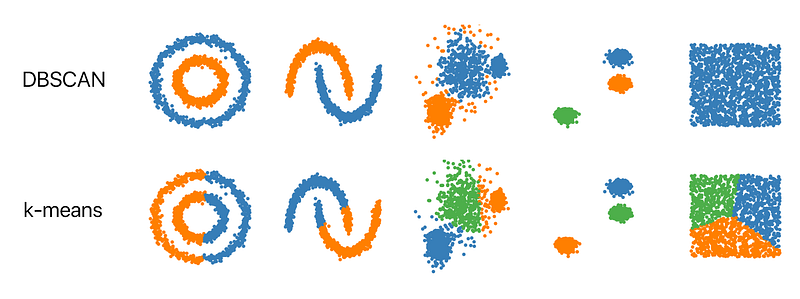
\includegraphics[width=0.8\textwidth]{chapters/聚类分析/images/DBSCAN-密度聚类/img-20250902154230.png}
\end{figure}

\begin{definition}[DBSCAN-密度聚类]
    密度聚类（DBSCAN）是一种无需事先指定聚类数量的聚类算法。通过不断扩展核心点的邻域，将所有密度相连的核心点划分为同一个聚类。对于边界点，如果它属于某个核心点的邻域内，但本身不是核心点，则被划分到该核心点所属的聚类中。最终，不属于任何核心点邻域的样本点被标记为噪声。

    DBSCAN基于“密度”的概念来定义聚类。简单来说，聚类是由密集区域中的点组成的，稀疏区域则被视为噪声。三个关键定义:
    \begin{enumerate}
        \item 核心点: 如果一个点周围在指定的半径（称为 $\epsilon$）内，至少有一定数量（minPts）的点，那么这个点就是核心点。核心点是聚类的“中心”。其中，邻域为：
              $$N_\epsilon(p)=\{q \in D \mid d(p, q) \leq \epsilon\}$$
              $$\text{p is a Core Point if} \left|N_\epsilon(p)\right| \geq \mathrm{MinPts}$$
        \item 边界点: 如果一个点在核心点的邻域内，但自身不是核心点，那么这个点是边界点。边界点靠近核心点，但不是密集区域的中心。
              $$
                  \mathrm{q} \text { is a Border Point if }\left|N_\epsilon(q)\right|<\operatorname{MinPts} \text { and } \exists p,\left(p \text { is a Core Point and } q \in N_\epsilon(p)\right)
              $$
        \item 噪声点: 如果一个点既不是核心点，也不是边界点，那么它被视为噪声点，属于离群点。
    \end{enumerate}
\end{definition}

\begin{warning}
    \begin{enumerate}
        \item Eps和MinPts是全局参数，难以处理不同密度的簇。
        \item 该模型对参数很敏感，需要不断调整参数达到较好的聚类效果；
        \item 该模型在高维数据中表现不佳，可能面临“维度灾难”。
    \end{enumerate}
\end{warning}

\begin{tips}
    \href{https://www.bbbdata.com/text/344}{https://www.bbbdata.com/text/344}
\end{tips}

\subsection{OPTICS 算法}

为了解决 DBSCAN 的全局参数的局限性，可以解决参数设置困难的问题。此时引入了两个核心概念：

\begin{definition}[核心距离]
    对于点 $p$ ，若其邻域内有足够点（ $\geq M i n P t s$ ），则核心距离为 $p$ 到其第 MinPts 近邻的距离。若邻域内不足 MinPts 个点，则核心距离未定义（无穷大）。
\end{definition}

\begin{definition}[可达距离]
    对于点 $A$ 和 $B, B$ 相对于 $A$ 的可达距离是 $A$ 的核心距离和 $A$ 到 $B$ 的欧氏距离之间的较大值。
    $$
        \text{reachability\_distance}(A, B)=\max(\text{core\_distance}(A), \text{distance}(A, B))
    $$
    直观理解：可达距离衡量了从一个点到另一个点＂被密度连接＂的难易程度。
\end{definition}

OPTICS通过类似DBSCAN的过程对数据进行排序，优先处理核心距离小的点（更密集区域）。输出一个"可达距离图"，通过观察＂山谷＂（低可达距离区域）识别簇。

但是，复杂性很高，簇的提取也很困难，需要手动观察可达距离图，还需要指定 \verb`minPts`，而且可达距离是不对称的。

\subsection{HDBSCAN 层次化的密度聚类}

\begin{definition}[HDBSCAN]
    引入了相对密度的概念，可以动态地通过互达距离，定义点之间的密度连接关系，更稳健。

    \textbf{密度层次化聚类}：
    \begin{itemize}
        \item 通过跟踪密度逐步降低的过程，生成密度分层树。
        \item 树的叶子节点代表高密度簇，根节点代表整个数据集。
    \end{itemize}

    \textbf{自动化簇提取}：提供自动化的簇提取方法，通过稳定性指标评估簇的持久性。

    \begin{tips}
        解决的问题：
        \begin{itemize}
            \item 密度差异问题：同一数据集中可能存在密度差异很大的聚类，简单使用原始距离可能导致低密度簇被忽略。
            \item 噪声数据识别问题：噪声点通常分布稀疏，与聚类距离较远，使用原始距离可能难以区分。
        \end{itemize}
    \end{tips}
\end{definition}

\begin{tips}
    所有具体算法的讲解在：\href{https://www.bilibili.com/video/BV1ktJizBEU6}{https://www.bilibili.com/video/BV1ktJizBEU6}
\end{tips}

\begin{theorem}[HDBSCAN 算法公式]

    \section{核心公式体系}
    \begin{enumerate}[label=\arabic*., wide, labelindent=0pt]
        \item \textbf{核心距离 (Core Distance)}:
              衡量点 $A$ 所在区域的局部密度，即点 $A$ 到其第 $k$ 个最近邻居的距离。
              $$
                  \text{core}_k(A) = \text{distance}(A, N^k(A))
              $$
        \item \textbf{相互可达距离 (Mutual Reachability Distance)}:
              算法最核心的公式。它是一种对称且经过密度平滑的距离度量，用于构建图的边权重。
              $$
                  d_{mreach}(A, B) = \max(\text{core}_k(A), \text{core}_k(B), \text{distance}(A, B))
              $$
        \item \textbf{构建最小生成树 (MST) 与聚类层级}:
              基于相互可达距离构建一个所有点的最小生成树，并依此生成聚类层级。
        \item \textbf{提取稳定簇}:
              通过计算每个潜在簇在层级中的“生命周期”或“稳定性”，自动选取最显著、最持久的簇作为最终结果，而非使用固定的距离阈值切割。
    \end{enumerate}

    \begin{itemize}[leftmargin=*, label=\textbullet]
        \item \textbf{能处理密度不均的簇}:
              最大的优点。能同时识别数据集中的高密度和低密度区域，而无需牺牲一方。
        \item \textbf{无需设置 \texttt{eps} 参数}:
              摆脱了 DBSCAN 中最难调节的 \texttt{eps} 参数，算法通过稳定性分析自动寻找最佳聚类。
        \item \textbf{参数更直观}:
              主要参数 \texttt{min\_cluster\_size}（簇的最小样本数）的物理意义清晰，易于根据业务背景设定。
        \item \textbf{噪声识别更鲁棒}:
              基于簇的稳定性进行判断，能更准确地区分真实噪声点和因密度波动形成的“伪簇”。
    \end{itemize}


\end{theorem}

\begin{lstlisting}[style=python]

\end{lstlisting}

\subsection{快速多核低维欧几里得空间的 HDBSCAN 算法}

\begin{definition}
    \verb`fast_hdbscan` 库提供了 HDBSCAN 聚类算法的简单实现，该算法专为在多核机器上处理低维数据（2 维到 20 维左右）而设计，以实现高性能。该算法并行运行，可以有效利用任意数量的内核来解决问题。因此，它非常适合大型 SMP 系统，甚至是现代多核笔记本电脑。

    \begin{tips}
        \href{https://github.com/TutteInstitute/fast_hdbscan/}{https://github.com/TutteInstitute/fast\_hdbscan/}
    \end{tips}
\end{definition}

\subsection{采用 DBSCAN 对高维向量采用余弦相似度聚类}

\begin{definition}
    对高维数据（例如来自语言模型的嵌入）进行聚类面临着独特的挑战。与需要预先指定聚类数量的 K-Means 算法不同，此代码库提供了一种使用 DBSCAN 算法的高级解决方案——这是一种适应性更强、洞察力更强的方法，尤其适用于大型复杂数据集。
\end{definition}

\begin{tips}
    \href{https://github.com/yigitkonur/hdbscan-embeddings-clustering}{https://github.com/yigitkonur/hdbscan-embeddings-clustering}
\end{tips}

